
%(BEGIN_QUESTION)
% Copyright 2006, Tony R. Kuphaldt, released under the Creative Commons Attribution License (v 1.0)
% This means you may do almost anything with this work of mine, so long as you give me proper credit

Calculate values for the following calibration table, for a transmitter measuring liquid level interface (specific gravities = 0.75 and 1.2), with a calibration tolerance of $\pm$ 0.1\%.  Be sure to specify which port on the $\Delta$P transmitter to apply the calibration pressure:

$$\includegraphics[width=15.5cm]{i00311x01.eps}$$

% No blank lines allowed between lines of an \halign structure!
% I use comments (%) instead, so that TeX doesn't choke.

$$\vbox{\offinterlineskip
\halign{\strut
\vrule \quad\hfil # \ \hfil & 
\vrule \quad\hfil # \ \hfil & 
\vrule \quad\hfil # \ \hfil & 
\vrule \quad\hfil # \ \hfil & 
\vrule \quad\hfil # \ \hfil & 
\vrule \quad\hfil # \ \hfil \vrule \cr
\noalign{\hrule}
%
% First row
Interface & Percent of & $\Delta$ pressure & Output signal & Output signal & Output signal \cr
%
% Another row
level (in) & span (\%) & sensed ("W.C) & ideal (mA) & min. (mA) & max. (mA) \cr
%
\noalign{\hrule}
%
% Another row
  & 0 &  &  &  &  \cr
%
\noalign{\hrule}
%
% Another row
  & 10 &  &  &  &  \cr
%
\noalign{\hrule}
%
% Another row
  & 25 &  &  &  &  \cr
%
\noalign{\hrule}
%
% Another row
  & 50 &  &  &  &  \cr
%
\noalign{\hrule}
%
% Another row
  & 75 &  &  &  &  \cr
%
\noalign{\hrule}
%
% Another row
  & 90 &  &  &  &  \cr
%
\noalign{\hrule}
%
% Another row
  & 100 &  &  &  &  \cr
%
\noalign{\hrule}
} % End of \halign 
}$$ % End of \vbox

\vskip 10pt

Be sure to show all your mathematical work so that your instructor will be able to check the conceptual validity of your technique(s).  A good way to check to see if you're solving the problem correctly is to check that each and every one of your intermediate calculations (i.e. the results you get mid-way during the process to arrive at the final answer) has real physical meaning.  {\bf If you truly understand what you are doing, you will be able to identify the correct unit of measurement for every intermediate result and also be able to show where that number applies to the scenario at hand}.


\vskip 20pt \vbox{\hrule \hbox{\strut \vrule{} {\bf Suggestions for Socratic discussion} \vrule} \hrule}

\begin{itemize}
\item{} Does the position of the transmitter within the 30 inch span matter?  For example, would the calibration be affected if the transmitter were re-located just 5 inches higher, without moving the remote seals?  Why or why not?
\item{} Suppose the process vessel were not filled all the way up to the overflow point.  How would this change affect the accuracy of the level transmitter?  Would it register falsely low, falsely high, or would it still register as it should?
\item{} Demonstrate how to {\it estimate} numerical answers for this problem without using a calculator.
\end{itemize}

\underbar{file i00311}
%(END_QUESTION)





%(BEGIN_ANSWER)

{\bf Partial answer:}

% No blank lines allowed between lines of an \halign structure!
% I use comments (%) instead, so that TeX doesn't choke.

$$\vbox{\offinterlineskip
\halign{\strut
\vrule \quad\hfil # \ \hfil & 
\vrule \quad\hfil # \ \hfil & 
\vrule \quad\hfil # \ \hfil & 
\vrule \quad\hfil # \ \hfil & 
\vrule \quad\hfil # \ \hfil & 
\vrule \quad\hfil # \ \hfil \vrule \cr
\noalign{\hrule}
%
% First row
Interface & Percent of & $\Delta$ pressure & Output signal & Output signal & Output signal \cr
%
% Another row
level (in) & span (\%) & sensed ("W.C) & ideal (mA) & min. (mA) & max. (mA) \cr
%
\noalign{\hrule}
%
% Another row
 & 0 & 10.5 L &  &  &  \cr
%
\noalign{\hrule}
%
% Another row
 & 10 &  & 5.6 &  &  \cr
%
\noalign{\hrule}
%
% Another row
7.5 & 25 &  &  &  &  \cr
%
\noalign{\hrule}
%
% Another row
 &  & 3.75 L &  &  &  \cr
%
\noalign{\hrule}
%
% Another row
 & 75 &  &  & 15.984 &  \cr
%
\noalign{\hrule}
%
% Another row
 & 90 & &  &  & 18.416 \cr
%
\noalign{\hrule}
%
% Another row
30 & 100 &  & &  &  \cr
%
\noalign{\hrule}
} % End of \halign 
}$$ % End of \vbox

Note: the letter ``L'' following the differential pressure value represents that amount of positive pressure applied to the {\it low} port of the transmitter.

%(END_ANSWER)





%(BEGIN_NOTES)

\noindent
{\bf LRV condition}:

There will be 30 inches of light liquid (SG = 0.75) sensed by the transmitter's ``H'' port and 30 inches of fill fluid (SG = 1.1) sensed by the ``L'' port.  The differential pressure in the LRV interface condition will therefore be:

$$\hbox{DP}_{LRV} = \left(30 \hbox{ in} \over 1 \right) \left(0.75 \hbox{ in water} \over 1 \hbox{ in liquid} \right) - \left(30 \hbox{ in} \over 1 \right) \left(1.1 \hbox{ in water} \over 1 \hbox{ in liquid} \right) $$

$$\hbox{DP}_{LRV} = (22.5 \hbox{ "WC}) - (33 \hbox{ "WC}) = -10.5 \hbox{ "WC}$$

\vskip 10pt

\noindent
{\bf URV condition}:

There will be 30 inches of heavy liquid (SG = 1.2) sensed by the transmitter's ``H'' port and 30 inches of fill fluid (SG = 1.1) sensed by the ``L'' port.  The differential pressure in the LRV interface condition will therefore be:

$$\hbox{DP}_{LRV} = \left(30 \hbox{ in} \over 1 \right) \left(1.2 \hbox{ in water} \over 1 \hbox{ in liquid} \right) - \left(30 \hbox{ in} \over 1 \right) \left(1.1 \hbox{ in water} \over 1 \hbox{ in liquid} \right) $$

$$\hbox{DP}_{URV} = (36 \hbox{ "WC}) - (33 \hbox{ "WC}) = +3.0 \hbox{ "WC}$$


The two remote seal capillary tubes working together present a constant pressure of $-33$ "WC to the DP transmitter regardless of the transmitter's elevation compared to the process vessel.  If we raise the transmitter, the fill fluid's hydrostatic pressure applied to the ``L'' side decreases but is exactly matched by an identical increase in the fill fluid's suction (negative pressure) applied to the ``H'' side.

It should also be noted that any process liquid height above the upper remote seal is irrelevant, since that hydrostatic pressure will be applied equally to both ``H'' and ``L'' ports of the transmitter and will therefore cancel (i.e. any hydrostatic pressure above the upper remote seal is {\it common-mode} and therefore unregistered by the DP transmitter).

% No blank lines allowed between lines of an \halign structure!
% I use comments (%) instead, so that TeX doesn't choke.

$$\vbox{\offinterlineskip
\halign{\strut
\vrule \quad\hfil # \ \hfil & 
\vrule \quad\hfil # \ \hfil & 
\vrule \quad\hfil # \ \hfil & 
\vrule \quad\hfil # \ \hfil & 
\vrule \quad\hfil # \ \hfil & 
\vrule \quad\hfil # \ \hfil \vrule \cr
\noalign{\hrule}
%
% First row
Interface & Percent of & $\Delta$ pressure & Output signal & Output signal & Output signal \cr
%
% Another row
level (in) & span (\%) & sensed ("W.C) & ideal (mA) & min. (mA) & max. (mA) \cr
%
\noalign{\hrule}
%
% Another row
0 & 0 & 10.5 L & 4 & 3.984 & 4.016 \cr
%
\noalign{\hrule}
%
% Another row
3 & 10 & 9.15 L & 5.6 & 5.584 & 5.616 \cr
%
\noalign{\hrule}
%
% Another row
7.5 & 25 & 7.125 L & 8 & 7.984 & 8.016 \cr
%
\noalign{\hrule}
%
% Another row
15 & 50 & 3.75 L & 12 & 11.984 & 12.016 \cr
%
\noalign{\hrule}
%
% Another row
22.5 & 75 & 0.375 L & 16 & 15.984 & 16.016 \cr
%
\noalign{\hrule}
%
% Another row
27 & 90 & 1.65 H & 18.4 & 18.384 & 18.416 \cr
%
\noalign{\hrule}
%
% Another row
30 & 100 & 3.0 H & 20 & 19.984 & 20.016 \cr
%
\noalign{\hrule}
} % End of \halign 
}$$ % End of \vbox

Note that with the remote seals, fill fluid density does not have to be any particular minimum value as is the case with open ``wet'' legs.  Students should also note that the height of the transmitter itself is unimportant.

%INDEX% Measurement, interface level: calibration table

%(END_NOTES)


